
\section{Schr\"{o}dinger's Cat\label{SchrondingersCat}}
Schr\"{o}dinger's famous thought experiment was first discussed in a 1935 paper in the context of the EPR paradox and the inherent problems it raised for the Copenhagen interpretation.\footnote{For Schr\"{o}dinger's original reference to his thought experiment, see \cite{SchrondingerOrig}. For an English translation, see \cite{SchrondingerEnglish}.} According to the Copenhagen interpretation, given the Bell state 
\begin{equation}\tag{\ref{bell} revisited}
    \ket*{\Psi_{\text{Bell}}}=\frac{1}{\sqrt{2}}(\ket*{\uvbp{a}}_A\ket*{\uvbm{a}}_B-\ket*{\uvbm{a}}_A\ket*{\uvbp{a}}_B),
\end{equation}
there is no fact of the matter as to whether particle $q_A$ is spin up and particle $q_B$ is spin down (or vice versa) until an observation is made. 

Now the strange goings-on at subatomic level might not initially give us much cause for concern about the nature of reality. For one might say that although it is an interesting curiosity that facts about subatomic particles are a bit fuzzy, our observation of definite facts in everyday life should convince us that such fuzziness can be brought into focus when we zoom out from the subatomic level to the macroscopic level. That is, we might suppose that the very many indefinite things on the small scale average out to give us something definite on the large scale. However, the Schr\"{o}dinger's Cat thought experiment suggests that our confidence in there being definite facts at the macroscopic level is seriously undermined if the Copenhagen interpretation is correct. Schr\"{o}dinger himself described the scenario in his thought experiment as ridiculous\footnote{See \cite[p. 328]{SchrondingerEnglish}.} indicating that he didn't think we should doubt the definiteness of facts at the macroscopic level; rather, we should call into question the reasonableness of the Copenhagen interpretation. 

The Schr\"{o}dinger's cat thought experiment invites us to consider a scenario like the one depicted in (\ref{BellCollapse1}) and (\ref{BellCollapse2}), but instead of having two microscopic particles coupled together, we have a microscopic particle such as a radioactive atom coupled together with a macroscopic object such as a cat. Sch\"{o}dinger suggests how this might be done. A cat is enclosed in a steel chamber in which there is a Geiger counter that is directed towards a small radioactive source, so that in the course of an hour, there is a probability of $\frac{1}{2}$ that the Geiger counter will click indicating that one of the radioactive atoms has decayed, and there is a probability of $\frac{1}{2}$ that the Geiger counter doesn't click because none of the radioactive atoms decay over the course of an hour. The Geiger counter itself is hooked up to a relay such that if the Geiger counter clicks, it releases a hammer which shatters a small flask of hydrocyanic acid causing the cat to die. The two possibilities are depicted in figure \ref{deadlivecat}.
\begin{figure}[ht!]
    \captionsetup{justification=justified}
    \centering
    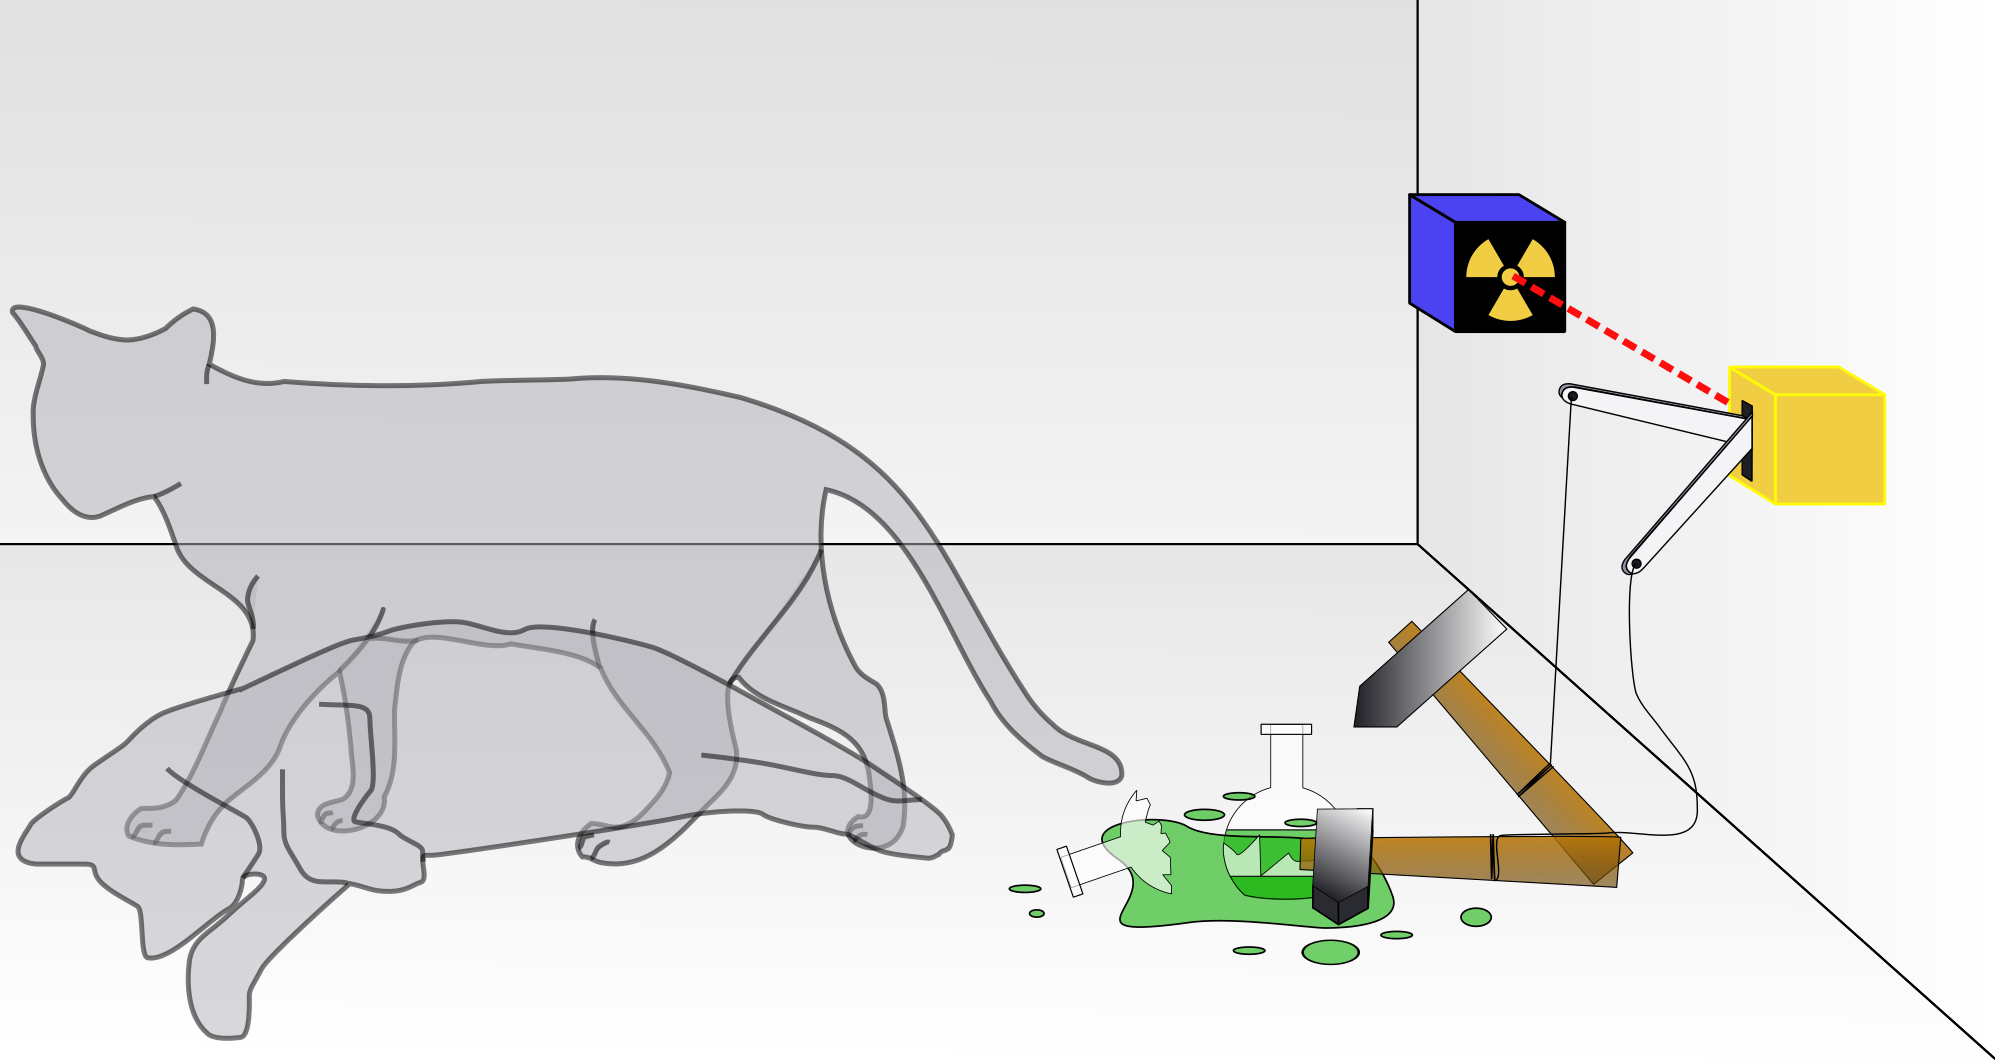
\includegraphics[width=100mm]{Chapter03/Schrodingers_cat.png}
    \caption[Caption for LOF]{A depiction of Schr\"{o}dinger's cat being both dead and alive.\protect\footnotemark}
    \label{deadlivecat}
    \end{figure}
    \footnotetext{ Original by Dhatfield. This image is licensed under the Creative Commons Attribution-Share Alike 3.0 Unported license. Source: https://commons.wikimedia.org/wiki/File:Schrodingers\_cat.svg}
    
    According to the Copenhagen interpretation, the cat will only enter into a determinate state once the box is opened at the end of the hour and an observation is made. Thus, there are two possibilities analogous to (\ref{BellCollapse1}) and (\ref{BellCollapse2}): either
\begin{equation*}
    \begin{split}
\frac{1}{\sqrt{2}}\Big(\ket*{\text{No atoms decay}}\ket*{\text{Cat Alive}}&-\ket*{\text{Atom decays}}\ket*{\text{Cat Dead}}\Big)\\
&\xrightarrow{\text{Collapse!!}}\ket*{\text{No atoms decay}}\ket*{\text{Cat Alive}},
\end{split}
\end{equation*}
or
\begin{equation*}
\begin{split}
\frac{1}{\sqrt{2}}\Big(\ket*{\text{No atoms decay}}\ket*{\text{Cat Alive}}&-\ket*{\text{Atom decays}}\ket*{\text{Cat Dead}}\Big)\\
&\xrightarrow{\text{Collapse!!}}\ket*{\text{Atom decays}}\ket*{\text{Cat Dead}}.
\end{split}
\end{equation*}
But before the box is opened and any measurement is made, the state of the cat and the atom will not be determinate, just as in the case of the spin-singlet where the spin states of the two particles are not determined to a definite value before any measurement is made. The Schr\"{o}dinger's Cat thought experiment thus highlights that under the Copenhagen interpretation, there is no good reason to restrict  indeterminacy to the microscopic level. If there is any indeterminacy at the microscopic level, then we should expect it at the macroscopic level as well, in which case it should be possible for a cat to be in an indeterminate state of being alive and dead. It is this possibility that Schr\"{o}dinger found ridiculous. 





